\section{Statistical methods} \label{sec:npde}

\subsection{Models and notations}

\hskip 18pt Let B denote a learning dataset and V a validation dataset. B is used to build a population pharmacokinetic model called M$^B$.

Let $i$ denote the i$^{\rm th}$ individual ($i$ = 1,..., N) and $j$ the j$^{\rm th}$ measurement in an individual 
($j$ = 1,..., n$_i$, where n$_i$ is the number of observations for subject $i$). Let Y$_i$=$\{y_{i1},...,y{in_i} 
\}$ be the n$_i$-vector of observations observed in individual $i$. Let the function $f$ denote the nonlinear 
structural model. $f$ can represent for instance the pharmacokinetic model. The statistical model for the 
observation $y_{ij}$ in patient $i$ at time t$_{ij}$, is given by: 
\begin{equation} 
y_{ij}=f(t_{ij},\theta_i)+\epsilon_{ij} 
\end{equation} 
where $\theta_i$ is the p-vector of the individual 
parameters and $\epsilon_{ij}$ is the residual error, which is assumed to be normal, with zero mean. The variance 
of $\epsilon_{ij}$ may depend on the predicted concentrations $f(t_{ij},\theta_i)$ through a (known) variance 
model. Let $\sigma$ denote the vector of unknown parameters of this variance model.

In pharmacokinetic (PK)/pharmacodynamic (PD) studies for instance, it is usually assumed that the variance of the 
error follows a combined error model: 
\begin{equation} 
\var(\epsilon_{ij})= (\sigma_{\rm inter} + \sigma_{\rm slope} \; f(t_{ij},\theta_i))^2 \label{eq:errormod} 
\end{equation} 
where $\sigma_{\rm inter}$ and $\sigma_{\rm 
slope}$ are two parameters characterising the variance. In this case, $\sigma=(\sigma_{\rm inter},\sigma_{\rm 
slope})'$. This combined variance model covers the case of an homoscedastic variance error model, where 
$\sigma_{\rm slope}=0$, and the case of a constant coefficient of variation error model when $\sigma_{\rm 
inter}=0$. Another parameterisation often found is: 
\begin{equation} 
\var(\epsilon_{ij})= \sigma_{\rm inter}^2 +  \sigma_{\rm slope}^2 \; f(t_{ij},\theta_i)^2 
\end{equation}

Another usual assumption in population PK/PD analyses is that the distribution of the individual parameters 
$\theta_i$ follows a normal distribution, or a log-normal distribution, as in: 
\begin{equation} 
\theta_i=h(\mu,  X_i) \; e^{\eta_i} \label{eq:modelPKcov} 
\end{equation} 
where $\mu$ is the population vector of the parameters, 
$X_i$ a vector of covariates, $h$ is a function giving the expected value of the parameters depending on the 
covariates, and $\eta_i$ represents the vector of random effects in individual $i$. $\eta_i$ usually follows a 
normal distribution $\mathcal{N} (0, \Omega)$, where $\Omega$ is the variance-covariance matrix of the random 
effects, but other parametric or non-parametric assumptions can be used for the distribution of the random effects, 
as in the first paper using this method, in the context of non-parametric estimation~\cite{Mesnil}. Although npde 
were developed in the context of pharmacokinetic and pharmacodynamic analyses, it is a general approach that can be 
used to evaluate mixed effect models. The key assumption is to be able to simulate from the expected model, and the 
npde are designed to test whether simulations and observations correspond.

We denote ${\rm \Psi}$ the vector of population parameters (also called hyperparameters) estimated using the data 
in the learning dataset B: ${\rm \Psi}= (\mu, \vec(\Omega),\sigma)'$, where $\vec(\Omega)$ is the vector of unknown 
values in $\Omega$. Model M$^B$ is defined by its structure and by the hyperparameters $\hat{\rm \Psi}^B$ estimated 
from the learning dataset B.

\subsection{Computing pde and npde in the absence of BQL data} \label{subsec:npdenoBQL}

\hskip 18pt Evaluation methods compare the predictions obtained by M$^B$, using the design of V, to the 
observations in V. V can be the learning dataset B (internal validation) or a different dataset (external 
validation). The null hypothesis (H$_0$) is that data in the validation dataset V can be described by model M$^B$. 
Prediction distribution errors are a metric designed to test this assumption. In this section, we assume that there 
is no observation below the limit of quantification (LOQ) in the validation dataset; an extension to BQL data is 
presented in section~\ref{sec:npdeBQL}.

\subsubsection{Prediction discrepancies (\pd)}

\hskip 18pt Let p$_{i}(y|\Psi)$ be the whole marginal posterior predictive distribution of an observation $y$ for 
the individual \emph{i} predicted by the tested model. p$_i$ is defined as: $$p_{i}(y|\Psi)=\int 
p(y|\theta_{i},\Psi) p(\theta_{i}|\Psi)d\theta_{i}$$

Let F$_{ij}$ denote the cumulative distribution function (cdf) of the predictive distribution p$_{i}(y|\Psi)$. The 
prediction discrepancy is defined as the percentile of an observation in the predictive distribution 
p$_{i}(y|\Psi)$, as given by: 

$$\pd_{ij}=F_{ij}(y_{ij})=\int^{y_{ij}} p_{i}(y|\Psi)dy=\int^{y_{ij}}\int 
p(y|\theta_{i},\Psi)p(\theta_{i}|\Psi)d\theta_{i}dy$$

In NLMEM, F$_{ij}$ has no analytical expression and can be approximated by MC simulations. Using the design of the 
validation dataset V, we simulate $K$ datasets V$^{sim(k)}$ ($k$=1,...,K) under model M$^B$. Let Y$_i^{sim(k)}$ 
denote the vector of simulated observations for the $i^{\rm th}$ subject in the $k^{\rm th}$ simulation. 

The prediction discrepancy $\pd_{ij}$ for observation y$_{ij}$ can then be computed from the cdf F$_{ij}$, as: 
\begin{equation} 
\pd_{ij} = F_{ij}(y_{ij}) \approx \frac{1}{K}{\textstyle \overset{K}{\underset{k=1}{\sum}}\boldsymbol{1}_{ \{y_{ij}^{sim(k)}<y_{ij} \}}} \label{eq:pdedef} 
\end{equation} To 
handle extreme values of the observations (defined as values smaller or larger than all the simulated values 
y$_{ij}^{sim(k)}$), we further set: 
\begin{equation*} 
\pd_{ij} = \left\{ 
\begin{array}{l r} \frac{1}{2K} & \text{if } y_{ij} \leq y_{ij}^{sim(k)} \; \forall \; k=1\ldots K \\ 
1-\frac{1}{2K} & \text{if } y_{ij} > y_{ij}^{sim(k)} \; \forall \; k=1\ldots K \\ 
\end{array} \right. 
\end{equation*} 
Under H$_0$, if $K$ is large enough, prediction 
discrepancies ($\pd$) follow $\mathcal{U}(0, 1)$ by construction.

\paragraph{Smoothing the distribution:} the simulation-based computation described above can lead to ties 
especially at the extremes, that is, different observations may have the same value of \pd~(this occurs 
particularly often if the number of simulations is small, or the model is quite different from the data). To avoid 
this issue, we have implemented an option to smooth the distribution: instead of using directly the quantile of the 
observation within the simulated distribution, as in equation~\ref{eq:pdedef}, we draw the \pd~randomly between 
this quantile (say $k/K$) and the one immediately above ($(k+1)/K$). We do this by adding a sample from a uniform 
distribution over the interval $\left[0,\frac{1}{K}\right]$ to the value defined by the previous equation: 
\begin{equation} 
\pd_{ij} = u_{ij} + \frac{1}{K}{\textstyle \overset{K}{\underset{k=1}{\sum}}\boldsymbol{1}_{y_{ij}^{sim(k)}<y_{ij}}} 
\end{equation} 
Again, extreme values of 
the observations are treated separately: 
\begin{equation*} 
\pd_{ij} \sim \left\{ 
\begin{array}{l r} 
U[0,1/K] &  \text{if } y_{ij} \leq y_{ij}^{sim(k)} \; \forall \; k=1\ldots K \\ 
U[1-1/K,1] & \text{if } y_{ij} >  y_{ij}^{sim(k)} \; \forall \; k=1\ldots K \\ 
\end{array} \right. 
\end{equation*} 
This option can be set by using the \texttt{ties=FALSE} argument.

\subsubsection{Prediction distribution errors (\pde)} 

\hskip 18pt When multiple observations are available for one subject, typically in population analyses, the $\pd$ 
are correlated within each subject~\cite{MentrePDE}. To correct for this correlation, we compute the mean 
$\mathbb{E}(\Y_i)$ and variance $\var(\Y_i)$ of the $K$ simulations. The mean is approximated by: 
$$\mathbb{E}(\Y_{i})\thickapprox\frac{1}{K}\overset{K}{\underset{k=1}{\sum}}\Y_{i}^{sim(k)}$$ and the 
variance-covariance matrix is approximated by: $$\var(\Y_{i})\thickapprox 
\frac{1}{K}\overset{K}{\underset{k=1}{\sum}}(\Y_{i}^{sim(k)}-E(\Y_{i}))(\Y_{i}^{sim(k)}-E(\Y_{i}))'$$ Decorrelation 
is performed simultaneously for simulated data: $$ \Y_{i}^{sim(k)*}= \var(\Y_i)^{-1/2} 
(\Y_{i}^{sim(k)}-\mathbb{E}(\Y_i))$$ and for observed data: $$ \Y_{i}^*= \var(\Y_i)^{-1/2} 
(\Y_{i}-\mathbb{E}(\Y_i))$$ Since we are looking to obtain 'residuals', different decorrelation options exist to 
obtain $\var(\Y_i)^{-1/2}$, corresponding to different sets of decorrelated data. In the \npde~package, we propose 
3 options, which will be detailed in the next section (section~\ref{subsec:decorrelation}).

Decorrelated $\pd$ are then obtained using the same formula as~\ref{eq:pdedef} but with the decorrelated data, and 
we call the resulting variables prediction distribution errors ($\pde$): 
\begin{equation} 
\pde_{ij} = F^*_{ij}(y^*_{ij}) 
\end{equation}

Under H$_0$, if $K$ is large enough, the distribution of the prediction distribution errors should follow a uniform 
distribution over the interval [0,1] by construction of the cdf. Normalized prediction distribution errors 
($\npde$) can then be obtained using the inverse function of the normal cumulative density function implemented in 
most software: 
\begin{equation} 
\npde_{ij} = \Phi^{-1} (\pde_{ij}) 
\end{equation}

By construction, if H$_0$ is true, $\npde$ follow the $\mathcal{N}(0, 1)$ distribution and are uncorrelated within 
an individual. The decorrelation step however does not make the $\npde$ truly independent, since this is only valid 
for Gaussian variables and here the model nonlinearity makes this only approximately true~\cite{Comets10}.

\subsubsection{Decorrelating the data to obtain \pde} \label{subsec:decorrelation}

\paragraph{Decorrelation methods:} To calculate the matrix $\var(\Y_i)^{-1/2}$ used for decorrelating data, we can 
use different methods.

The Cholesky decomposition is a standard way to obtain residuals in regression models, and was used in the initial 
implementation of the \npde~library. It is computationally simple, numerically stable, and remains the default 
method. However, as an iterative pivotal algorithm it is sensitive to the ordering of the vector of $\Y_i$. In PK 
or PD applications, time imposes a natural order on the vector of longitudinal observations which makes this method 
very relevant, however this may not be as simple for instance when there are multiple responses. The Cholesky 
decomposition method is also used in the proc MIXED of SAS, to calculate residuals for correlated data. Let 
$\mathrm{C}$ denote the Cholesky root of $\var(\Y_i)$ so that $$\mathrm{C}'\mathrm{C} = \var(\Y_i)$$ Then 
$\var(\Y_i)^{-1/2} = (\mathrm{C}')^{-1}$. 

Using a Cholesky decomposition is not the only way to define residuals. An alternative which is invariant to 
re-ordering of the vector of observations is to use the unique square root of the matrix $\var(\Y_{i})$, obtained 
using an eigenvalue decomposition. The matrix $\var(\Y_i)$ can be factorized as: $\var(\Y_{i})= \mathrm{Q} \Lambda 
\mathrm{Q}^{-1}$, where Q is the square matrix of the same dimension of $\var(\Y_i)$, whose i\textsuperscript{th} 
column is the eigenvector of $\var(\Y_i)$ and $\Lambda$ is the diagonal matrix whose diagonal elements are the 
corresponding eigenvalues. The square root matrix of $\var(\Y_i)$ is then calculated as: $$\var(\Y_i)^{1/2} = 
\mathrm{Q} \Lambda^{1/2} \mathrm{Q}^{-1}$$ and this square root matrix is inverted to calculate the matrix 
$\var(\Y_i)^{-1/2}$. This method is currently implemented in MONOLIX 4 and NONMEM 7 to calculate weighted residuals 
(WRES, IWPRES) and npde. However, when calculating the symmetric square root from the eigen value-eigen vector 
decomposition, we will essentially be defining principle directions determined by the variance-covariance matrix 
and thus, the decorrelated observations/residuals are rotated and no longer correspond to the natural ordering.

We have also implemented a third method, combining a Cholesky decomposition with a polar 
decomposition~\cite{Higham86}. Let $\mathrm{C}$ denote the Cholesky root of $\var(\Y_i)$. Using polar 
decomposition, the matrix $\mathrm{C}$ can be factorized as: $\mathrm{C} = \mathrm{U} \mathrm{H}$, where U is a 
unitary matrix and H is a positive-semidefinite Hermitian matrix. The square root matrix of $\var(\Y_i)$ is then 
calculated as: $$\var(\Y_i)^{1/2} = \mathrm{U}' \mathrm{C}$$ This square root matrix is then inversed to calculate 
the matrix $\var(\Y_i)^{-1/2}$.

% ECO TODO: interêt de la décomposition polaire ?

\paragraph{Choosing a decorrelation method:} The Cholesky method was the only option available in the previous 
version of the library (npde 1.2) and is implemented as the default method in the current version (npde 2.0). 
Choosing the decorrelation method is done using the \texttt{decorr.method=""} option, with the following choices: 
\begin{center} 
\begin{tabular}{c p{11cm}} 
\hline decorr.method="cholesky" & Cholesky decomposition (pseudo-inverse  obtained by the \texttt{chol} function)\\ 
decorr.method="inverse" & Inverse (unique inverse, obtained using the \texttt{eigen} function)\\
decorr.method="polar" & polar decomposition (pseudo-inverse obtained by combining the \texttt{chol} function with the \texttt{svd} function)\\ 
\hline 
\end{tabular} 
\end{center} 
\begin{description} 
\item[{\bf Note:}] The user needs to be aware that sometimes the decorrelation step (regardless of the method 
chosen to perform it) will induce or mask patterns in the graphs of $\npde$ versus time or predictions. When 
strange patterns are seen, we advise the user to also look at the $\pd$ graphs, which do not involve the 
decorrelation step, to ascertain whether these patterns are really due to model misspecification and not an 
artefact of the decorrelation step, and/or to test different decorrelation methods. 
\end{description}

\subsection{Handling BQL data} \label{sec:npdeBQL}

\paragraph{Choosing the method to handle BQL data:} BQL data means that we do not observe $y_{ij}$ directly, but 
that we know the observation to be below a censoring value. We restrict ourselves to data below the LOQ, although 
extension to interval-censored data is straightforward. BQL data in the validation dataset can be treated in 
different ways: 
\begin{itemize} 
\item removed from the dataset: option {\sf cens.method = "omit"} 
\item imputed to model predictions: population predictions (option {\sf cens.method = "ppred"}) or individual predictions (option {\sf cens.method = "ipred"}) 
    \begin{itemize} 
    \item with the \texttt{"ppred"} method, population predictions are computed using the simulated datasets (for observation $y_{ij}$, the population prediction is $E_k(y^{sim(k)}_{ij})$)) 
    \item with the \texttt{"ipred"} method, individual predictions for each observation obtained during the estimation process need to be included in the data file as an additional column 
    \item $\pd$ and $\npde$ are computed after replacing observed and simulated data by the imputed values 
    \end{itemize} 
\item imputed  to a fixed value: to LOQ (option {\sf cens.method = "loq"}) or to a value chosen by the user (option {\sf cens.method = "fixed",loq=LOQ} where LOQ is a number) 
    \begin{itemize} 
    \item as in the previous method, $\pd$ and $\npde$ are computed after replacing observed and simulated data by the imputed values 
    \end{itemize} 
\item imputed using the cumulative density function: option {\sf cens.method = "cdf"}; this is a slightly more complex method in which we use the expected probability to be below LOQ to define $\pd$ and impute data based on the imputed $\pd$; it is detailed separately below. 
\end{itemize} 
Sometimes the data includes different LOQs (for 
instance when the dataset pools several studies with different analytical methods). In this case, the program 
computes the smallest LOQ in the dataset, and this value is used to censor the simulated data (eg, any simulated 
value in the dataset lower than the LOQ is omitted or replaced using the imputation method chosen).

Note that all methods involve some loss of power, all the more important when the fraction of BQL data is large, 
and thus conclusions must be made with prudence when using these imputation methods. However, simulations show that 
the {\sf cens.method = "cdf"} is the most suitable~\cite{Nguyen2012}, and that methods imputing directly with a 
fixed value or with population model predictions have a poor performance.

% ECO TODO: Tram, vrai aussi pour methode ipred ?

\paragraph{Imputation of BQL data using the cumulative distribution function)~\cite{Nguyen2012}:} this is the 
default option, which can also be explicit by using {\sf cens.method = "cdf"} in the call to the function.

For an observation above LOQ, the $\pd$ is computed as described above, as the quantile of the observation within 
the predicted distribution. For a BQL observation (left-censored observation) $y^{cens}_{ij}$ of the 
i\textsuperscript{th} individual at time $t_{ij}$, we first evaluate its probability of being under LOQ 
Pr$(y_{ij}^{cens}\leq\mbox{LOQ})$ using the predictive distribution predicted from the model: 
\begin{equation} 
\Pr(y_{ij}^{cens}\leq\mbox{LOQ})=F_{ij}(\mbox{LOQ})=\frac{1}{K}{\textstyle 
\overset{K}{\underset{k=1}{\sum}}\boldsymbol{1}_{y_{ij}^{sim(k)}\leq\mbox{LOQ}}} 
\end{equation} 
(these predicted probabilities are stored and returned in the results, see section~\ref{sec:npde.methods}). Since 
we only know that the actual observation is below LOQ, we propose to compute the $\pd$ for a left-censored 
observation y$_{ij}^{cens}$, pd$_{ij}^{cens}$, as a random sample from a uniform distribution over the interval 
[0,Pr$(y_{ij}^{cens}\leq\mbox{LOQ})]$.

To obtain the $\npde$ however, we first need to also impute observations which are below LOQ. We transform the 
imputed $\pd$ back to an imputed observation using the inverse function of the predictive distribution function 
$F_{ij}$: \begin{equation} y_{ij}^{cens(new)}=F_{ij}^{-1}(pd_{ij}^{cens}) \end{equation} Since $\pd$ are quantiles, 
this corresponds to finding the quantile immediately after the imputed $\pd_{ij}$ and setting $y_{ij}^{cens(new)}$ 
to the value in the simulated distribution $F_{ij}$ corresponding to that quantile (see figure~\ref{fig:imputation} 
for an illustration). The new vector of observations Y$_{i}^{new}$ now contains both observed values, for non 
censored data, and imputed values for censored data. 

\begin{figure}[!h] 
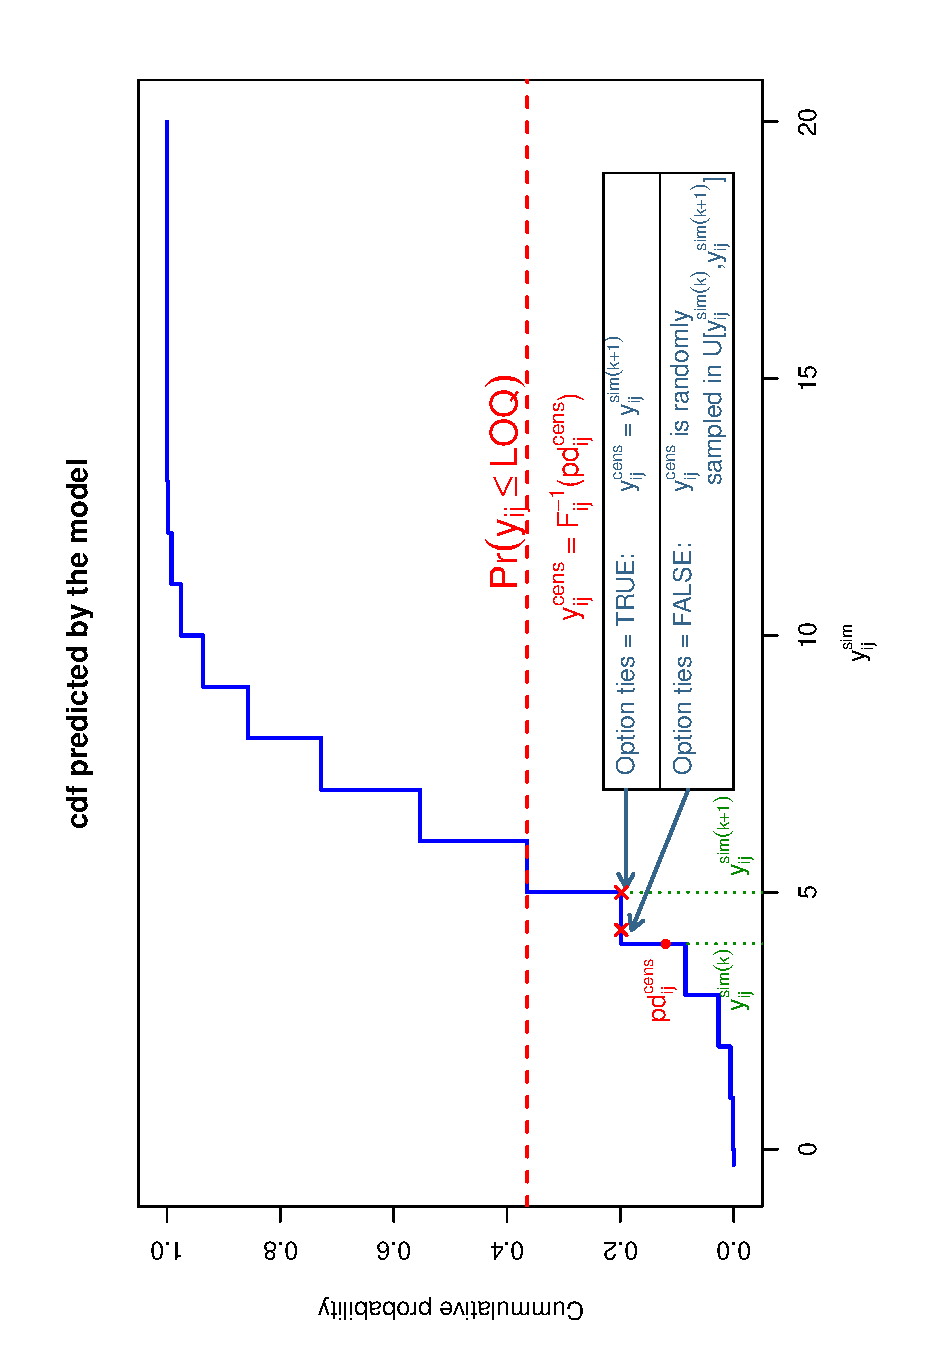
\includegraphics[angle=270,scale=0.7]{figs/imputation.eps} 
\caption{Imputation y$_{ij}^{cens}$ from pd$_{ij}^{cens}$ and F$_{ij}$ with the two options {\sf "ties = TRUE"} and 
{\sf "ties = FALSE"}} \label{fig:imputation} 
\end{figure}

We cannot simply decorrelate the vector of observed data $y_{i}$ using the simulations from the model, because the 
simulated dataset also contains values that would have been censored and treating them as simulated. We therefore 
propose to impute these censored data to a value between 0 and LOQ using the same method. We impute a 
pd$_{ij}^{sim(new),k}$ for each y$_{ij}^{sim,k}$ below LOQ in the simulated data and these y$_{ij}^{sim,k}$ are 
replaced using the same imputation method applied to the observed data. \begin{equation} 
y_{ij}^{sim(new),k}=F_{ij}^{-1}(pd_{ij}^{sim(new),k})\,\,\,\mbox{if }y_{ij}^{sim}\leq LOQ \end{equation}

\bigskip As previously, to avoid ties in the $\pd$ and $\npde$, we can jitter the imputed $\pd$ and $y$. 
Figure~\ref{fig:imputation} shows an illustration for both cases: \begin{itemize} \item method {\sf "ties = TRUE"}: 
if $F_{ij}(y_{ij}^{sim(k)}) < pd_{ij}^{cens}\leq F_{ij}(y_{ij}^{sim(k+1)})$, then $y_{ij}^{cens} = 
y_{ij}^{sim(k+1)}$ \item method {\sf "ties = FALSE"}: if $F_{ij}(y_{ij}^{sim(k)}) < pd_{ij}^{cens}\leq 
F_{ij}(y_{ij}^{sim(k+1)})$, then $y_{ij}^{cens}$ is randomly sampled in a uniform distribution over the interval 
[$y_{ij}^{sim(k)},y_{ij}^{sim(k+1)})$] \end{itemize}

After the imputation step, a new vector of observations Y$_{i}^{new}$ and new simulated data Y$_{i}^{sim_{new}}$ 
are obtained. The complete data are then decorrelated using the same technique as described above. Note that the 
ma!!trix $\var(\Y_i)$ used to decorrelate is computed using the imputed data, while the predictive distribution 
functions $F_{ij}$ are computed using the original simulated data before the imputation step.

\subsection{Tests}

\subsubsection{Tests on the distribution of npde} \hskip 18pt Under the null hypothesis that model M$^B$ describes 
adequately the data in the validation dataset, the $\npde$ follow the $\mathcal{N}(0, 1)$ distribution. We report 
the first three central moments of the distribution of the $\npde$: mean, variance, skewness, as well as the 
kurtosis, where we define kurtosis as the fourth moment minus 3 so that the kurtosis for $\mathcal{N}(0,1)$ is 0 
(sometimes called excess kurtosis). The expected value of these four variables for the expected $\mathcal{N}(0,1)$ 
are respectively 0, 1, 0 and 0. We also give the standard errors for the mean (SE=$\sigma/\sqrt{N}$) and variance 
(SE=$\sigma \; \sqrt{2/(N-1)}$).

We use 3 tests to test the assumption that the $\npde$ follow the $\mathcal{N}(0, 1)$ distribution: (i) a Wilcoxon 
signed rank test, to test whether the mean is significantly different from 0; (ii) a Fisher test for variance, to 
test whether the variance is significantly different from 1; (iii) a Shapiro-Wilks test, to test whether the 
distribution is significantly different from a normal distribution. The package also reports a global test, which 
consists in considering the 3 tests above with a Bonferroni correction~\cite{Brendel10}. The p-value for this 
global test is then reported as the minimum of the 3 p-values multiplied by 3, the number of simultaneous tests (or 
1 if this value is larger than 1)~\cite{Wright}. A graphical code is used in the library to highlight significant 
results, similar to the code used by other statistical functions in {\sf R} such as {\sf lm} (see example). The 
normality test is very powerful, especially with large amount of observations. When the test remains significant 
even after model refinement, QQ-plots should be used to assess model adequacy in addition to the 3 statistical 
tests. This is especially useful in large datasets where the sheer amount of data will lead to reject even 
reasonable models.

\subsubsection{Tests for covariate models} 

\hskip 18pt In~\cite{Brendel10}, we proposed two approaches to evaluate a model with or without covariates with a 
validation dataset. 

In the first approach, for continuous covariates we can test for correlations between the covariate and $\npde$, 
using the Spearman correlation test; for categorical covariates we can use Wilcoxon or Kruskal-Wallis tests. If the 
model and validation data correspond, there should be no relationship between $\npde$ and covariates.

In the second approach, we proposed to split the $\npde$ according to the values of the covariate, and test within 
each category that $\npde$ follows a $\mathcal{N}(0,1)$ distribution. For categorical covariates, $\npde$ are split 
by categories of the covariate. We proposed to discretise continuous covariates in 3 classes, below first quartile 
($<$Q$_1$), between first and third quartiles (Q$_1$--Q$_3$) and above third quartile ($>$Q$_3$). If the model and 
validation data correspond, there should be no significant departure from $\mathcal{N}(0,1)$ within each category: 
a test is performed for each category, and the resulting p-values are corrected with a Bonferroni correction.

Both approaches gave similar results in terms of type I error in a simulation study, but the second approach has a 
slightly larger type I error and a correspondingly slight increase in power~\cite{Brendel10}. Tests for covariate 
models will be added shortly to the library.

\subsection{Graphs} \label{sec:graphmethods}

Table~\ref{tab:plot.type} shows the different plots which can be created using the {\sf plot.type} argument.

\subsubsection{Diagnostic graphs} 

\paragraph{Assessing the distribution of npde:} Graphs can be used to visualise the shape of the distribution of 
the $\npde$. Classical plots include quantile-quantile plots (QQ-plots) of the distribution of the $\npde$ against 
the theoretical distribution, as well as  histograms and empirical cumulative distributions of the $\npde$ and 
$\pd$. We also find that scatterplots of the $\npde$ versus the independent variable, the predicted dependent 
variables, or covariates, can help pinpoint model deficiencies. Some of these graphs are plotted by default (see 
section~\ref{sec:graphics}). The package computes for each observation the predicted value as the empirical mean 
over the $k$ simulations of the simulated predicted distribution (denoted $E_k(y^{sim(k)}_{ij})$), which is 
reported under the name $\ypred$ along with the $\npde$ and/or $\pd$.

In the field of population PK/PD, graphs of residuals versus predictions use the values predicted by the model even 
when the residuals have been decorrelated, as is the case for both spe and npde here. Comparing metrics to their 
theoretical distributions can be done through QQ-plots or histograms [10]. Examples of these different graphs will 
be shown in the next section.

\paragraph{Probability of being under the LOQ:} Finally, when the dataset includes data below the LOQ, a plot of 
the probability of being BQL can be useful to assess whether the model is able to adequately predict low values, 
and is available in the \npde~package.

\paragraph{Prediction intervals:} In the current version of the library, prediction bands around selected 
percentiles, which can be obtained through repeated simulations under the model being tested, can be added to most 
graphs to highlight departures from predicted values~\cite{Comets10}. Prediction intervals build on the idea of 
simulating from the model to evaluate whether it can reproduce the observed data. For the VPC, a 95\% prediction 
interval on a given percentile (eg the median) can be obtained by computing the median for the K simulated datasets 
and taking the region where 95\% of these K medians lie. This can also be applied to scatterplots of $\npde$ or 
$\pd$, where for each percentile plotted in the graph we can compute a prediction interval of a given size. By 
default, 95\% is used in the \npde~package, and each prediction interval is plotted as a coloured area (blue for 
the 2.5 and 97.5th percentile and pink for the median); the corresponding 2.5th, 50th and 97.5th percentiles of the 
observed data are plotted as lines or points, and should remain within the coloured areas.

A binning algorithm is used for the prediction intervals (the number of bins can be adjusted by the user). 
Different options are: (1) equal bin sizes on the X-axis; (2) equal bin widths on the X-axis; (3) optimal binning 
using a clustering algorithm to select the optimal breaks; (4) user-selected breaks. The binning algorithm uses the 
\texttt{Mclust} library~\cite{Fraley02,Fraley06} for \texttt{R}, which implements model-based clustering with an 
EM-algorithm to select the optimal number of clusters for the variable on the X-axis of the graph.

\subsubsection{Graphs for covariate models} 

\hskip 18pt Two types of diagnostic graphs are available in the {\sf npde} library for covariates. First, all the 
graphs can be split according to the values of the covariate, to examine the $\npde$ separately in each group. We 
use the representation proposed in~\cite{Brendel10} to evaluate covariate models, where $\npde$ are split by 
category for discrete covariates or by quantiles for continuous covariates (by default, 3 quantiles are used, 
$<Q1$, interquartile range $Q1-Q3$ over the middle 50\% value of the covariate, and $>Q3$, but the user can select 
the number of pertinent categories relative to the problem at hand). Prediction bands are also added to those 
graphs. These graphs can be obtained using the corresponding {\sf plot.type} argument (for instance, {\sf 
plot.type='x.scatter'} for a graph of $\npd$ versus the predictor) in conjunction with the argument {\sf 
covsplit=TRUE}; the covariates over which to split are specified as a vector of name using the argument {\sf 
which.cov} (defaults to all covariates).

A second type of diagnostic is to plot the $\npde$ or $\npd$ versus covariates, to examine the trends. For 
continuous covariates, a scatterplot of the metrics versus the covariate is provided, while for categorical 
covariates, we show boxplots for the different categories. Graphs of the metrics versus covariates can be produced 
using {\sf plot.type='cov.scatter'}.

\subsubsection{VPC} 

\hskip 18pt Visual Predictive Check (VPC) are standard diagnostic graphs that are now available also in the {\sf 
npde} library. In contrast to $\npde$, they do not handle heterogeneity in the design (eg dose regimen) or 
covariates, so that they are most useful in balanced designs to evaluate models without covariates. However since 
they are directly obtained from model observations and predictions they illustrate very nicely the shape of the 
evolution of independent versus dependent variable. VPC are obtained by simulating repeatedly under the model and 
plotting selected percentiles of the simulated data, comparing them to the same percentiles in the observed data. 
By default, the VPC produced in the \npde~package correspond to the median and limits of the 95\% prediction 
interval (eg, the 2.5th, 50th and 97.5th percentile of the data). The observed data can also be plotted over the 
interval, or omitted for very large datasets.

In the presence of censored data, the same imputation method is also applied to the VPC. For instance, with the 
default method ({\sf cens.method='cdf'}), the data under the LOQ is set to the value imputed from the predictive 
distribution through the imputed $\pde$, as described in methods, for {\sf cens.method='ipred'} it it replaced by 
the corresponding individual predictions (which then have to be given in the dataset), while for {\sf 
cens.method='omit'}, it is removed from the dataset. In this last case, the simulated data used to compute the 
prediction bands is also removed from the simulated dataset, yielding larger prediction bands reflecting the lower 
number of observations involved. VPC are produced using the argument {\sf plot.type='vpc'}.

\paragraph{Stratification:} when the model contains covariate effects, traditional VPC should be stratified and 
examined in each group. Alternatively, corrections such as pcVPC have been proposed, but are not implemented in the 
{\sf npde} library. 

\subsubsection{Graphs with a reference profile}

\hskip 18pt A new feature of the {\sf npde} library is the ability to add a reference plot to the scatterplot of 
$\npde$ or $\npd$ versus the independent variable. This was first described in a poster at the PAGE 
conference~\cite{CometsPAGE13}, and makes the $\npde$ plots similar in aspect to VPC, with information on both the 
evolution of the process and the distribution of residuals in the same plot. 

The principle is to first select a reference profile, which can be associated with a subject or a group of subject, 
a covariate or combination of covariates. We then distribute the $\npde$ (or the $\npd$) around this reference 
profile, taking into account the interindividual variability. To do this, we first compute for each value $x_t$ of 
the predictor $x$ the mean $\mathbb{E}_{t_{ij}}$ and standard deviation SD$_{t_{ij}}$ of the simulations 
corresponding to the selected reference profile for that time. Denoting $I_R$ the set of individuals corresponding 
to the reference profile, we compute:

\begin{equation} 
\begin{split} 
\mathbb{E}_{t_{ij}} &= \frac{1}{I_R \; K} \sum_{k=1}^{K} \sum_{i \in I_R}  y_{ij}^{sim(k)} \\ 
{\rm Var}_{t_{ij}} &=  \frac{1}{I_R \; K -1}  \sum_{k=1}^{K} \sum_{i \in I_R}  (y_{ij}^{sim(k)} - \mathbb{E}_{t_{ij}})^2 \\ 
\end{split} 
\end{equation}

We then compute the transformed $\npde$ at time $t_{ij}$ as: \begin{equation} \tnpde_{ij} = \mathbb{E}_{t_{ij}} + 
{\rm SD}_{t_{ij}} \; \npde_{ij} \end{equation} This is performed for each time point for a balanced design. In the 
case of an unbalanced design, we first bin the predictors on the $X$ axis~\cite{Lavielle11} and we compute the mean 
and SD for each bin, which are used within each bin to compute the transformed $\npde$. If the reference profile 
doesn't cover all the bins, we interpolate the missing values from the means and SD estimated in the available 
bins. 

We then produce plots of $\tnpde$ versus the predictor as previously, for a given interval size (eg 90\% prediction 
intervals), by computing the observed and simulated percentiles of the $\tnpde$ on the observed and simulated data 
respectively. Prediction intervals around the percentiles can be obtained by the same transformation.

Finally, we can apply the same procedure to transform the $\npd_{ij}$, bearing in mind the $\tnpd_{ij}$ will retain 
the correlation due to repeated observations.

The plots generated with a reference profile have a similar interpretation as VPC, but since they are based on 
$\npde$, there should be no correlation between the different $\tnpde$ for a subject. A minor difference in 
construction is that VPC plot the median and extreme percentiles (eg 5$^{\rm th}$ and 95$^{\rm th}$ percentiles for 
a 90\% VPC), while with $\tnpde$ we translate the median of the residual plots by the mean of the reference 
profile, and expand the extreme percentiles using the standard deviation. 

Note that it is the user's responsibility to use a pertinent reference profile. For example, if the design 
contains different dose-groups, the reference profile should be computed across one of the doses. In addition, the 
{\sf npde} library offers an option to set a different reference profile for each value of a covariate when 
splitting the scatterplot over covariates (see previous section).

% Larger PI than with VPC

\paragraph{Non-parametric construction of $\tnpde$:} an alternative using the median and quantiles of the 
reference profile to transform the $\npde$ will be implemented shortly.

% Under the null hypothesis, we expect pde to follow the distribution  $\mathcal{U}[0,1]$ and npde to follow the distribution $\mathcal{N}(0,1)$. It should be noted that left-censored observations in the validation datasets are imputed using the model to be evaluated, which could lead to loss of power if the model is wrong.	
